\documentclass{beamer}
\usepackage[utf8]{inputenc}
\usepackage{graphicx}
\usepackage{subfig}
\author[Sowmya Vajjala]{Instructor: Sowmya Vajjala}


\title[LING 120]{LING 120, Fall 2017 \\ Language and Computers}

\date{22 September 2017}

\institute{Iowa State University, USA}

%%%%%%%%%%%%%%%%%%%%%%%%%%%

\begin{document}

\begin{frame}\titlepage
\end{frame}

\begin{frame}
\frametitle{Class outline}%5minutes
\begin{enumerate}
\item Recap of last class
\item Searching the web: Ranking search results
\item Announcement: Midterm - teams and topics
\item Group Exercise on understanding search results
\item Reminder: Submit Assignment 2 on time!
\end{enumerate}
\end{frame} %\item Assignment 3 Description - do this on Monday

\begin{frame}
\frametitle{How does a search engine work?}
\framesubtitle{Which of those require some analysis of language?}
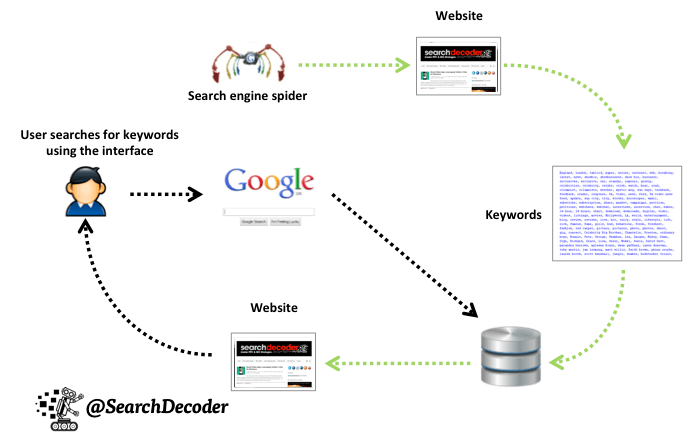
\includegraphics[width=0.9\textwidth]{search.png}
\medskip \tiny source: \url{https://www.searchdecoder.com/how-do-search-engines-work}
\end{frame}

\begin{frame}
\frametitle{TDM and Inverted Index}
%2 pictures.
\begin{figure}%
    \centering
    \subfloat[Term Document Matrix]{{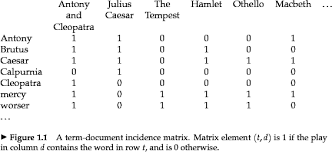
\includegraphics[width=5cm]{tdm.png} }}%
    \qquad
    \subfloat[Inverted Index]{{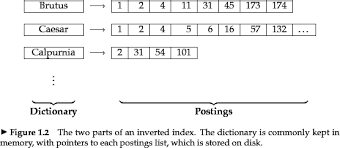
\includegraphics[width=5cm]{invertedindex.png} }}%
   % \caption{2 Figures side by side}%
    \label{fig:example}%
\end{figure}
\end{frame}

\begin{frame}
\frametitle{Questions to resolve Today}
\begin{itemize}
\item Okay, indexing is cool. But for any query, I may still end up with 10000 results. How can I rank them?
\item How do I ensure only good quality pages get ranked on top. 
\end{itemize}
\end{frame}

\begin{frame}
\frametitle{Ranking Search Results}
\begin{itemize}
\item Search engines use different kinds of information to rank web-pages. 
\item We briefly saw some of them in the last class (e.g., are the query words in the title of the web page? etc)
\item There can be several other factors such as: whether this page is "appropriate" for this user, whether this user previously spent long time on pages from this website etc. \pause
\item Note: Search engines know a lot about us. Much more than you think. (e.g., \url{https://goo.gl/cwQoGL})
\item 200 factors google uses: \url{https://backlinko.com/google-ranking-factors} (NOTE: This is not validated by Google) \pause
\item One popular ranking approach that was very influential in computer based search is: PageRank
\end{itemize}
\end{frame}

\begin{frame}
\frametitle{Page Rank}
\begin{itemize}
\item Intuition: If a page has a lot of other pages linking to it, it could mean the page is well-known, and is perhaps of good quality and is authoritaitve.
\item So, the "rank" a page has is determined by pages linking to it
\item ... and also the number of links into these pages as well. \pause
\item When the indexer returns two pages which are both relevant to a given query, one can then rank pages by their page rank and show to the user!
\end{itemize}
\end{frame}

%Understanding query: ambiguity issues in search
\begin{frame}
\frametitle{Other issues in search}
\begin{itemize}
\item Let us say someone started searching for "I love Java" - ideally, a search engine should cluster results into multiple "senses" of meaning - Java coffee, Java - the place, Java - the programming language. (Kind of difficult. Open question). \pause
\item Detecting pages with duplicate content \pause 
\item Working through multiple forms of data (if I give a query, how about getting back mp3 files containing that query as results??) 
\end{itemize}
... and so on.
%http://searchengineland.com/the-language-problem-jaguars-the-turing-test-92265
%http://www.seobythesea.com/2010/08/how-a-search-engine-might-interpret-ambiguous-queries-through-entity-tags/
\end{frame}

\begin{frame}
How google works:  \url{https://www.google.com/search/howsearchworks/algorithms/}
\end{frame}

\begin{frame}
\frametitle{Mid-term: Dates and Expectations}
\begin{itemize}
\item Dates: 9th-11th October
\item Teams (next slide) 1--3 on Monday (9th); 4--6 on Wednesday (11th) 
\end{itemize}
\end{frame}

\begin{frame}
\frametitle{Mid-term Groups}
\begin{enumerate}
\item Group 1: Dallas Evers, Krishna Chaitanya Gummalla, Nellie Waidelich, Congyu Zhao
\item Group 2: Marcelanne Gaebler, Gabriel Muhammed, Trevor Holbrook, Yangyifan Lu
\item Group 3: Nathan Friedrichsen, Linghan Zhang, Sydney Steinauer, Jordan Yardley
\item Group 4: Joseph Hudson, Brandon Huegli, Miles Lucas
\item Group 5: Maceo Jackson, Matthew Schaffer, Joshua Slagle
\item Group 6: Emily Kurimski, Dylan Mrzlak, Jonah McDermed, Ethan McGill
\end{enumerate}
\end{frame}

\begin{frame}
\frametitle{Mid-term Topics}
Uploaded on Canvas. 
11 topics in total - choose one of them. (Descriptions)
\end{frame}

\begin{frame}
\frametitle{Last class' Exercise}
Think about these problems and submit your thoughts online on Canvas forum for today. 
\begin{itemize}
\item Is "popularity" a good heuristic to rank a page? Provide one example where your search query results in a popular page as the top result, but is incorrect for your need. What is the rank of the page that met your need?
\item Question on Googlewhack. That website in the picture does not work though. You should use other means to know more.  
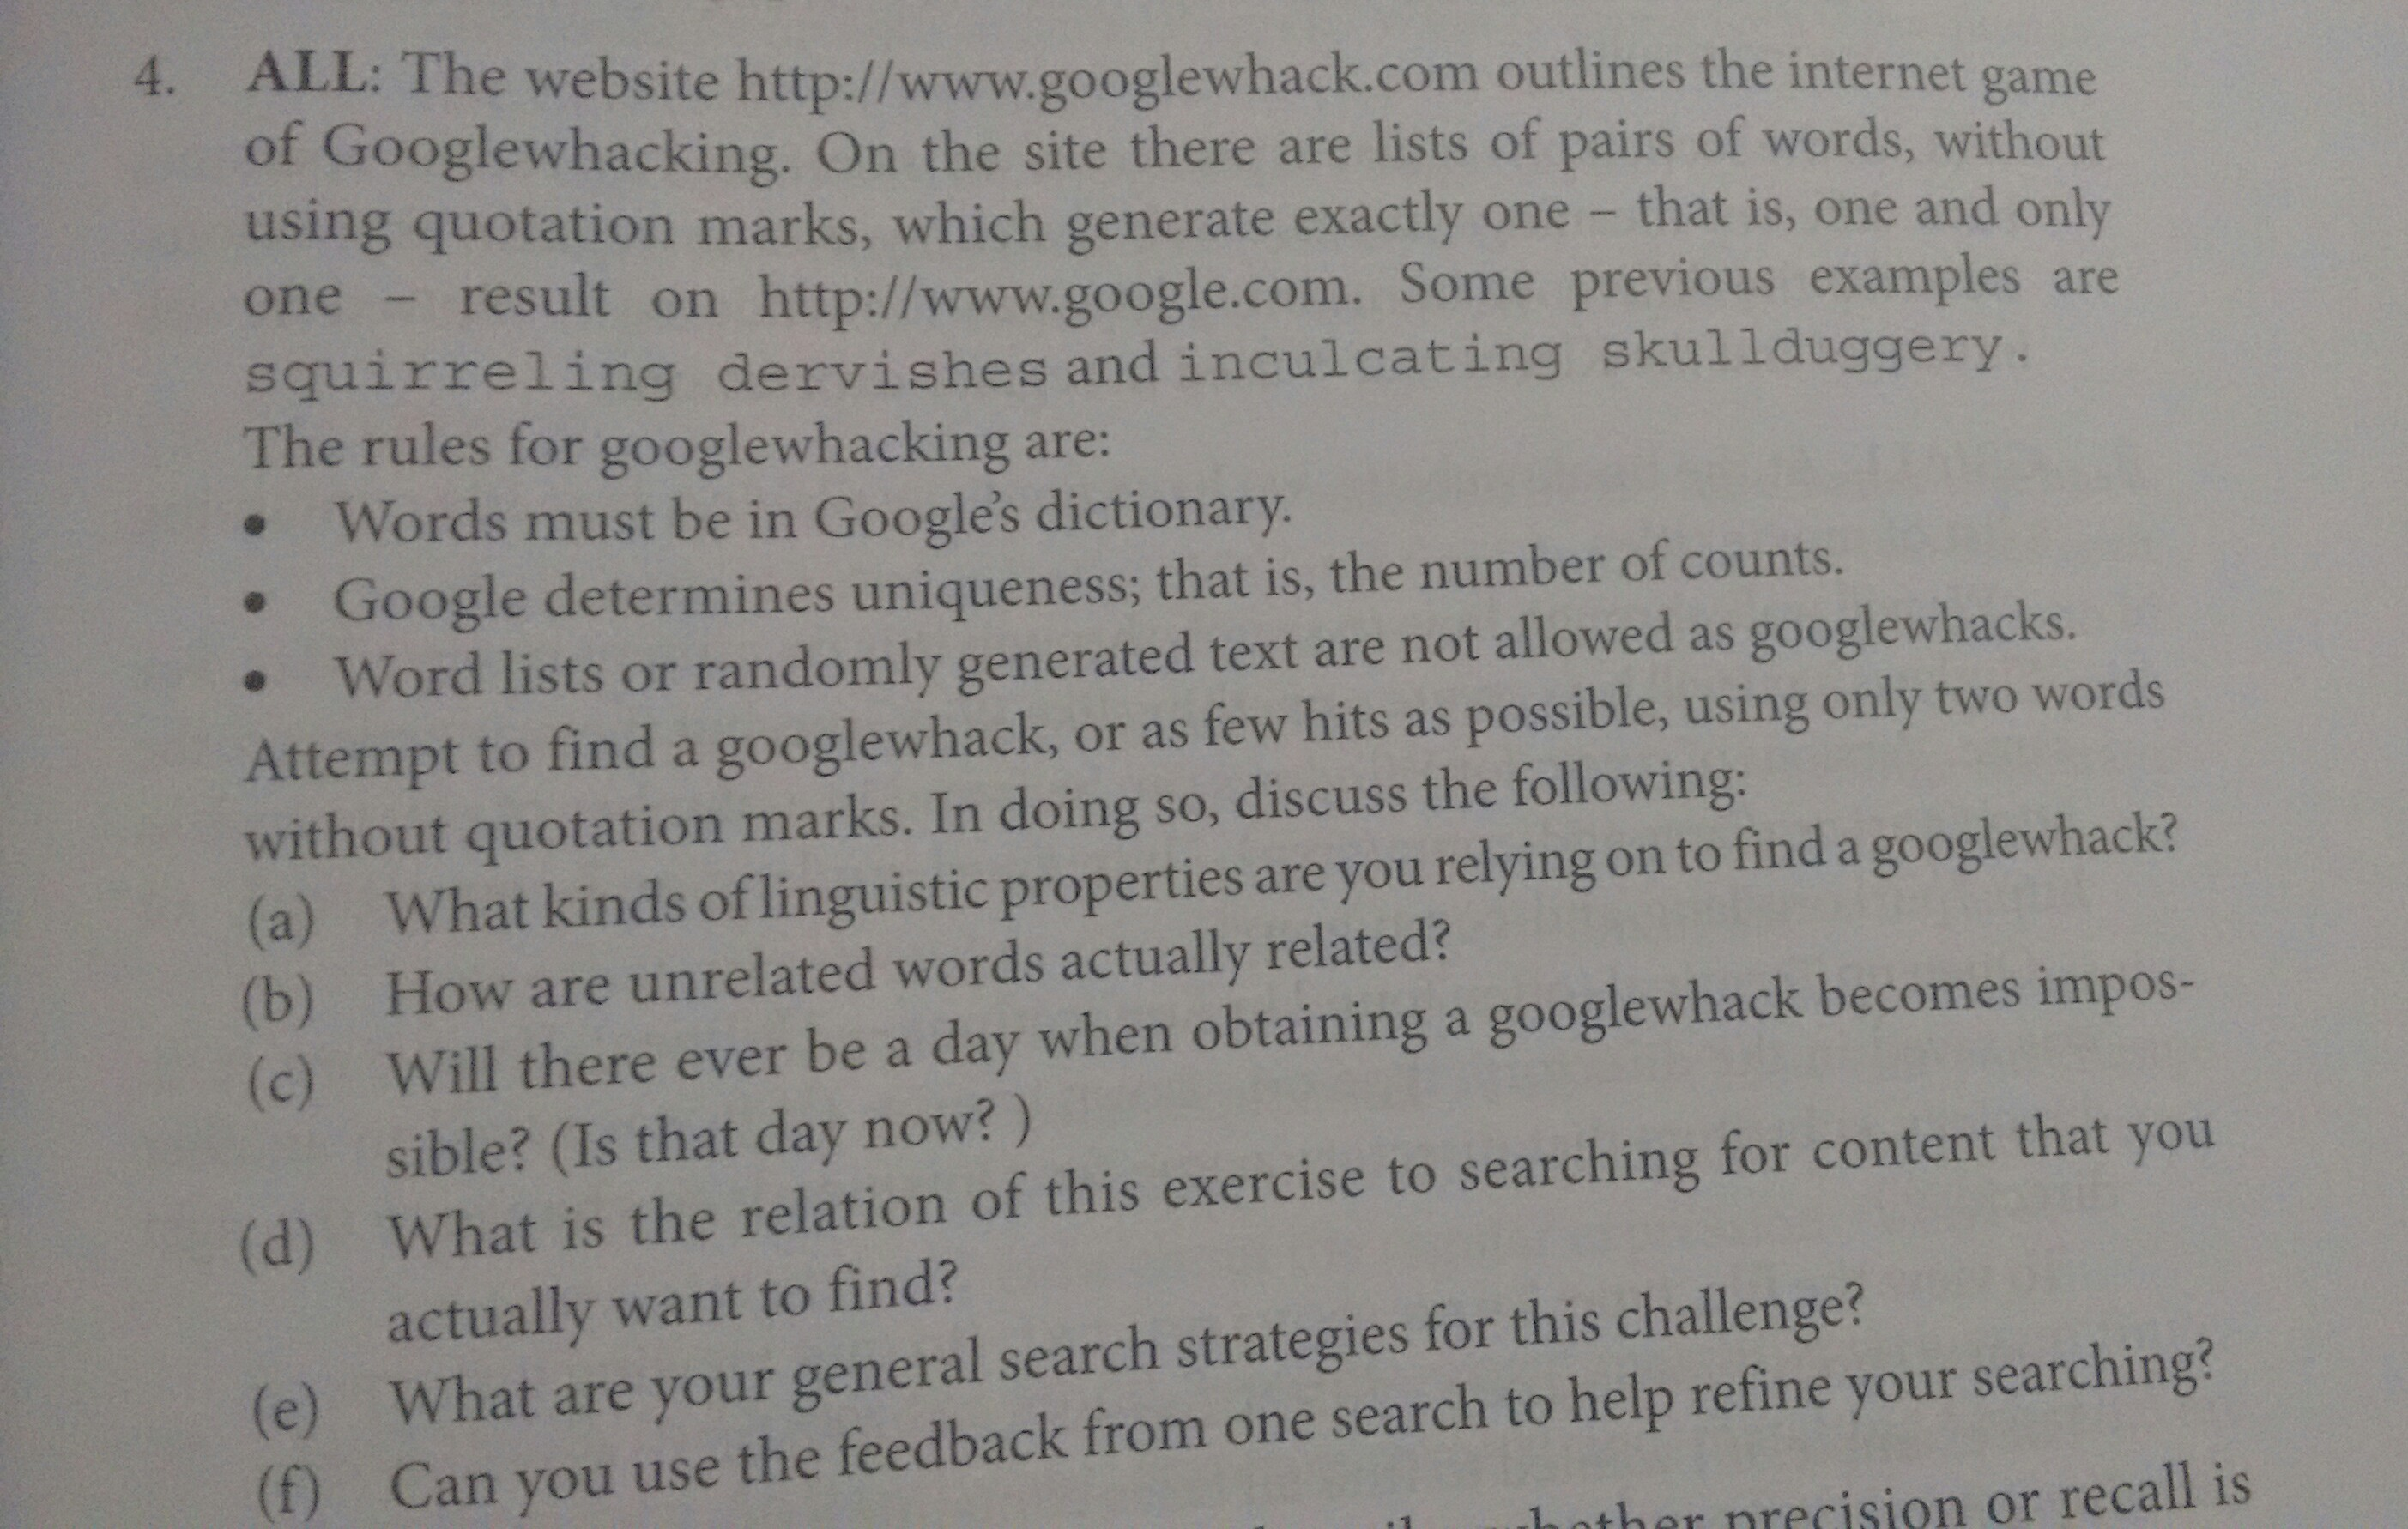
\includegraphics[width=0.6\textwidth]{20Sep-120Exercise.jpg}
\end{itemize}
\end{frame}

\begin{frame}
\frametitle{Attendance Exercise}
\begin{itemize}
\item Work in groups of 3 and submit a solution to the problem in the handout.
\item You can also submit this online on Canvas.
\item question url: \url{http://nacloweb.org/resources/problems/2007/N2007-B.pdf}
\end{itemize}
\end{frame}

\begin{frame}
\frametitle{Next Week}
\begin{itemize}
\item Semi-structured search, Regular Expressions
\item Assignment 3 Description and Assignment 2 Discussion (Monday) 
\item To do: Read Chapter 4, Finish Assignment 2
\item Could do: Know your mid-term team members. Start thinking about a topic.
\end{itemize}
\end{frame}

\end{document}
